\documentclass[aspectratio=169]{beamer}
\usetheme{default}
\usecolortheme{crane}
\setbeamertemplate{footline}{}
\setbeamertemplate{navigation symbols}{}

\usepackage{tikz, pgfplots}
\usetikzlibrary{positioning,arrows.meta}

\title{Nelder-Mead Simplex}
\subtitle{for Optimization}

\titlegraphic{\vspace{-2.1cm}
	\begin{center}
	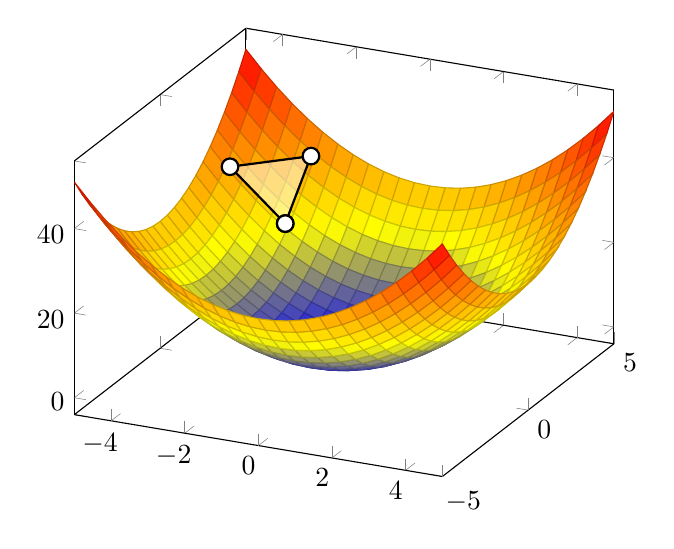
\begin{tikzpicture} 
		\begin{axis}
			\addplot3[surf]{1+x^2+y^2};
			\addplot3[mark=*,thick,black,fill=white,fill opacity=.5,mark options={fill=white, opacity=1, scale=1.5}] coordinates {(-3,3,19) (-3,4.5,30.25) (-4.5,3,30.25) (-3,3,19)};
		\end{axis}
	\end{tikzpicture}
	\end{center}
}

\date{}

\setbeamercolor{problem}{fg=black,bg=lime}

\begin{document}

	\begin{frame}
		\titlepage
	\end{frame}

	\begin{frame}
		\frametitle{Background}
		\textbf{Optimization} is the process of finding a combination of parameters that yields the ``best" result for a given problem.
		\begin{block}{Example}
			At what angle should a ball be thrown to travel the maximum distance away from you (in a vacuum)?
				\begin{center}
				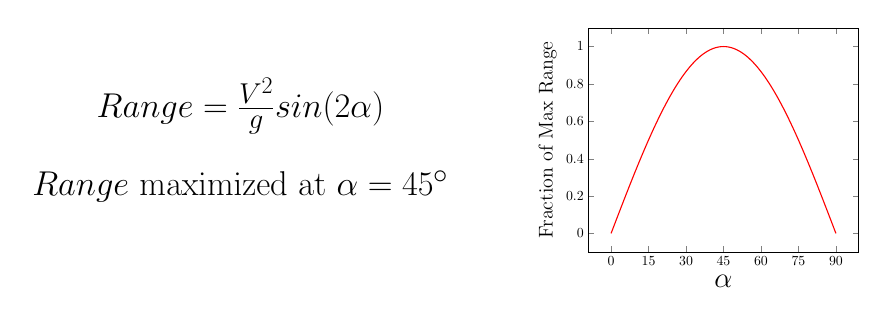
\begin{tikzpicture}[scale=0.5]
				\begin{axis}[extra description/.code={
						\node[anchor=east,align=center] (description1) at (-0.5,0.5) {\Huge$Range=\frac{V^2}{g}sin(2\alpha)$ \\ \\ \\ \\
						\Huge$Range$ maximized at $\alpha=45^{\circ}$};
					},
				xtick={0,15,30,45,60,75,90},
				xlabel=\huge$\alpha$,
				ylabel=\Large Fraction of Max Range]
				\addplot[domain=0:90,samples=50,smooth,red,thick] {sin(2*x)};
				\end{axis}
			\end{tikzpicture}
		\end{center}
		\end{block}
	\end{frame}

	\begin{frame}
		\frametitle{Background (cont)}
		The \textbf{objective function}, $f$, evaluates the quantity (or quantities) of interest as a function of the \textbf{design variables}, $x$. We usually try to minimize the objective function.
		$$ minimize \; f(x) $$
		$$	subject \; to \; x \in X $$
		where $X$ is the \textbf{design space} of the problem.\\
		\vspace{1cm}
		There are many iterative computational algorithms for optimization, including:
		\begin{itemize}
			\item gradient-based methods
			\item evolutionary methods
			\item other fancy math methods that make no sense
		\end{itemize}
	\end{frame}

	\begin{frame}
		\frametitle{Motivating Problem}
		\begin{beamercolorbox}[sep=1em]{problem}
			\textbf{\emph{Voices in your head}} indicate that treasure is buried at the deepest point in a local pond. With only a rowboat and a tape-measure to measure the depth of water below you, how might you find the treasure?\\
		\end{beamercolorbox}
		\vspace{0.5cm}
		Would you...
		\begin{itemize}
			\item Spend all night measuring the depth everywhere in the pond?
			\item Make an initial guess, perturb your guess East and North, compute the slopes, move some distance in the direction of maximum descent, and repeat until you can't find a deeper point?
			\item Make 3 initial guesses, make a 4th guess based on the others, throw away the worst of your 4 guesses, and repeat until you can't find a deeper point?
		\end{itemize}
	\end{frame}
	
	\begin{frame}
		\frametitle{Motivating Problem (cont)}
		\begin{center}
		Instead of taking physical measurements, we will evaluate:
		$$ Depth = f(x_1,x_2) = .006(x_1-1)^2+.009(x_2-2)^2+.005x_1 x_2-10 $$
		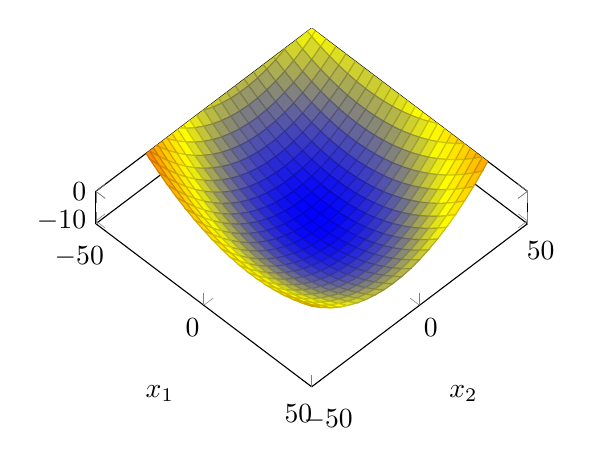
\begin{tikzpicture} 
			\begin{axis}[scale=0.8,
				xmin=-50,xmax=50,
				ymin=-50,ymax=50,
				zmax=0,
				ztick={-10,0},
				xlabel=$x_1$,
				ylabel=$x_2$,
				view={45}{82}]
				\addplot3[surf,domain=-50:50]{-10+.006*(x-1)^2+.009*(y-2)^2+.005*x*y};
			\end{axis}
		\end{tikzpicture}
		\end{center}
	\end{frame}

	\begin{frame}[fragile]
		\frametitle{Introduction to Nelder-Mead}
		Nelder-Mead is an iterative numerical method to find the (local) minimum or maximum of an objective function.\\[\baselineskip]
		
		For an optimization problem with $n$ variables, a simplex of $n+1$ points is created which gradually moves and contracts around the local optimal value. This method does not involve computing the derivatives/gradient of the objective function.\\[\baselineskip]
		
		A \textbf{simplex} is basically a generalization of what a triangle is in 2D space. For example, a simplex in 3D would be a tetrahedron, and a simplex in 1D would be a line segment.\\[\baselineskip]
		
		The algorithm is very simple to understand. I have adapted this explanation from the original paper by JA Nelder and R Mead, which is available for free online:\\[\baselineskip]
		
		\begin{verbatim}
		Nelder, J. A., & Mead, R. (1965). A Simplex Method for Function 
		Minimization. The Computer Journal, 7(4), 308-313.	
		\end{verbatim}
	\end{frame}

	\begin{frame}
		\frametitle{The Algorithm}
		I will explain the algorithm generically for a $n$-dimensional design space, but to help you visualize, I will illustrate the algorithm on a 2D design space (using a triangular simplex).\\[\baselineskip]
		
		We will attempt to find the local minimum of our objective function. If you would like to find a local maximum instead, negate the objective function:
		
		$$ maximize \; g(x) = minimize \; f(x)$$
		$$ for \; f(x)=-g(x) $$	
		
	\end{frame}

	\begin{frame}
		\frametitle{Step 0, Initialize Simplex}
		The zeroth step is to evaluate the initial vertices of the simplex. Evaluate the objective function at $n+1$ points:
		$$ P_0, P_1, P_2, \; ... \; P_n $$
		$$ P_i = \begin{bmatrix} x_1 & x_2 & ... & x_n \end{bmatrix}_i $$

		These points should ideally by centered close to our best guess of the optimum.		\\[\baselineskip]
		Keep in mind that this algorithm may only converge on a local optimum, and that may not in general be the global optimum. \\[\baselineskip]
		Let the function value at the vertices be represented by $y_i$ at point $P_i$:
		$$ y_i=f(P_i) $$
	\end{frame}

	\begin{frame}
		\frametitle{Step 0, Initialize Simplex (cont)}
		Here is how an initial simplex might look for our treasure-seeking problem:
		\begin{center}
			\begin{tikzpicture} 
				\begin{axis}[extra description/.code={
						\node[anchor=west,align=center] (description1) at (1.1,0.5) 
							{$P_0=\begin{bmatrix} -30 & 30 \end{bmatrix}$ \\ 
							 $y_0=f(P_0)=-1.678$ \\ \\
 							$P_1=\begin{bmatrix} -20 & 20 \end{bmatrix}$ \\ 
						 	$y_1=f(P_1)=-6.438$ \\ \\		 				
						 	$P_2=\begin{bmatrix} -10 & 30 \end{bmatrix}$ \\ 
						 	$y_2=f(P_2)=-3.718$
					 	};
					},
					scale=1,
					xmin=-50,xmax=50,
					ymin=-50,ymax=50,
					zmax=0,
					ztick={-10,0},
					xlabel=$x_1$,
					ylabel=$x_2$,
					view={45}{82},]
					\addplot3[surf,domain=-50:50]{-10+.006*(x-1)^2+.009*(y-2)^2+.005*x*y};
					\addplot3[mark=none,thick,black,fill=white,fill opacity=.5] coordinates {(-30,30,-1.678) (-20,20,-6.438) (-10,30,-3.718) (-30,30,-1.678)};
					\addplot3[mark=*,thick,black,text=white,mark options={fill=white, opacity=1, scale=1.5}, nodes near coords, point meta=explicit symbolic,    visualization depends on={value \thisrow{anchor}\as\myanchor},
					every node near coord/.append style={font=\small,anchor=\myanchor}] table [
					row sep=\\,
					meta=label
					]{
						x y z label anchor\\
						-30 30 -1.678 $P_0$ south\\
						-20 20 -6.438 $P_1$ east\\
						-10 30 -3.718 $P_2$ west\\
					};
				\end{axis}
			\end{tikzpicture}
		\end{center}
	\end{frame}


	\begin{frame}
		\frametitle{Step 0, Initialize Simplex (cont)}
		Because our task is to eventually find a $P_i$ associated with a local minimum $y_i$, we can compare the $y_i$ values that we have in order to get an idea of the direction in which the function $f$ is decreasing most.  \\[\baselineskip] 
		Obviously the $P_i$ associated with the highest (worst) $y_i$ is likely \textbf{NOT} in the direction of the optimum, whereas the $P_i$ associated with the lowest (best) $y_i$ \textbf{MAY BE} in the direction of the optimum.
		\\[\baselineskip] 
		Although it's not explicitly necessary, it may be useful to order the points $P_i$ by increasing/decreasing values of $y_i$ to help keep track of our point ranks.
	\end{frame}


	\begin{frame}
		\frametitle{Step 1, REFLECT}
		The first simplex transformation is basically to \textbf{REFLECT} the worst point of the simplex across the centroid defined by the other points. 
		\\[\baselineskip] 
		For simplicity, we will define $P_{best}$ and $P_{worst}$ as the best and worst points in the current simplex and $y_{best}$ and $y_{worst}$ as the corresponding function values.
		$$y_{best}=\min_{i} (y_i) = \min_{i} (f(P_i))  = f(P_{best})$$
		$$y_{worst}=\max_{i} (y_i) = \max_{i} (f(P_i)) = f(P_{worst})$$
		We also define $\bar{P}$ as the centroid of all but the worst points in the simplex:
		$$ \bar{P}=\frac{1}{n}\sum_{P_i\neq P_{worst}}P_i $$
	\end{frame}
	
	\begin{frame}
		\frametitle{Step 1, REFLECT (cont)}
		The new reflected simplex vertex $P^*$ can be expressed:
		$$P^*=(1+\alpha)\bar{P}-\alpha P_{worst} $$
		where $\alpha$ is a positive term called the \textbf{reflection coefficient} and is often taken to be $1$.
		\\[\baselineskip] 
		For $\alpha=1$, $\bar{P}$ is exactly between $P_{worst}$ and $P^*$. 
		\\[\baselineskip] 
		\begin{center}
		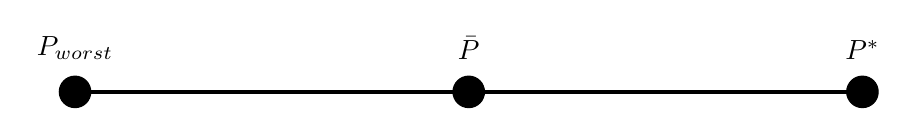
\begin{tikzpicture}
			\draw[ultra thick] (-5,0)--(0,0)--(5,0);
			\draw[black,fill=black](-5,0) circle [radius=0.2] node[above=8pt] {$P_{worst}$};
			\draw[black,fill=black]( 0,0) circle [radius=0.2] node[above=8pt] {$\bar{P}$};
			\draw[black,fill=black]( 5,0) circle [radius=0.2] node[above=8pt] {$P^*$};
		\end{tikzpicture}
		\end{center}
	Evaluate $y^*=f(P^*)$.
	\end{frame}
	
	\begin{frame}
		\frametitle{Step 1, REFLECT (cont)}
		Here is how a REFLECT operation might look for our treasure-seeking problem:
		\begin{center}
			\begin{tikzpicture} 
				\begin{axis}[extra description/.code={
						\node[anchor=west,align=center] (description1) at (1.1,0.5) 
						{$\bar{P}=\begin{bmatrix} -15 & 25 \end{bmatrix}$ \\ \\
							$P^*=\begin{bmatrix} 0 & 20 \end{bmatrix}$ \\ 
							$y^*=f(P^*)=-7.078$ 	 				
						};
					},
					scale=1,
					xmin=-50,xmax=50,
					ymin=-50,ymax=50,
					zmax=0,
					ztick={-10,0},
					xlabel=$x_1$,
					ylabel=$x_2$,
					view={45}{82},]
					\addplot3[surf,domain=-50:50]{-10+.006*(x-1)^2+.009*(y-2)^2+.005*x*y};
					\addplot3[mark=none,thick,black,fill=white,fill opacity=.5] coordinates {(-30,30,-1.678) (-20,20,-6.438) (-10,30,-3.718) (-30,30,-1.678)};
					\addplot3[mark=*,thick,black,text=white,mark options={fill=white, opacity=1, scale=1.5}, nodes near coords, point meta=explicit symbolic,    visualization depends on={value \thisrow{anchor}\as\myanchor},
					every node near coord/.append style={font=\small,anchor=\myanchor}] table [
					row sep=\\,
					meta=label
					]{
						x y z label anchor\\
						-30 30 -1.678 $P_0$ south\\
						-20 20 -6.438 $P_1$ east\\
						-10 30 -3.718 $P_2$ west\\
					};
					\addplot3[mark=*,thick,black,text=white,mark options={fill=white, opacity=1, 	scale=1.5}, nodes near coords, point meta=explicit symbolic,    visualization depends on={value \thisrow{anchor}\as\myanchor},
					every node near coord/.append style={font=\small,anchor=\myanchor}] table [
					row sep=\\,
					meta=label
					]{
						x y z label anchor\\
						-15 25 -5.578 $\bar{P}$ north\\
						0 20 -7.078 $P^*$ north\\
					};
				\end{axis}
			\end{tikzpicture}
		\end{center}
	\end{frame}

	\begin{frame}
		\frametitle{Step 1, REFLECT (cont)}
		There a few options for the value of $y^*$:\\[\baselineskip]
		\begin{itemize}
			\item $y* \leq y_{best}$ (the reflected point is the best so far):
			\begin{itemize}
				\item We should look further in the direction of $P^*$, continue to the \textbf{EXPAND} step.
			\end{itemize}
		\end{itemize}
		\begin{itemize}
			\item $y* \geq y_{2^{nd} worst}$ (if the reflected point replaced the worst point, it would still be the worst):
			\begin{itemize}
				\item Reflecting didn't work, and our simplex is likely too big. We should contract our existing simplex away from of $P_{worst}$, continue to the \textbf{CONTRACT} step.
			\end{itemize}
		\end{itemize}
		\begin{itemize}
			\item $y_{best}<y*<y_{2^{nd} worst}$ (the reflected point is at most second-worst):
			\begin{itemize}
				\item We can improve our simplex by replacing $P_{worst}$ with $P^*$. Do so, and if we haven't satisfied the \textbf{STOPPING CRITERIA}, return to the \textbf{REFLECT} step.
			\end{itemize}
		\end{itemize}
	\end{frame}

	\begin{frame}
		\frametitle{Step 2, EXPAND}
		The next simplex transformation is basically to \textbf{EXPAND} the reflected point $P^*$ on our simplex further in that direction. It helps us quickly traverse the design space in the direction of the expected minimum. 
		\\[\baselineskip]
		We define an expanded point $P^{**}$:
		$$P^{**}=\gamma P^*+(1-\gamma)\bar{P}$$
		where $\gamma$ is a term greater than $1$ called the \textbf{expansion coefficient} and is often taken to be $2$.
	\end{frame}

	\begin{frame}
		\frametitle{Step 2, EXPAND (cont)}
		Here is how an EXPAND operation might look for our treasure-seeking problem:
		\begin{center}
			\begin{tikzpicture} 
				\begin{axis}[extra description/.code={
						\node[anchor=west,align=center] (description1) at (1.1,0.5) 
						{$\bar{P}=\begin{bmatrix} -15 & 25 \end{bmatrix}$ \\ \\
							$P^*=\begin{bmatrix} 0 & 20 \end{bmatrix}$ \\ 
							$y^*=f(P^*)=-7.078$\\ \\
							$P^{**}=\begin{bmatrix} 15 & 15 \end{bmatrix}$ \\ 
							$y^{**}=f(P^{**})=-6.178$  				
						};
					},
					scale=1,
					xmin=-50,xmax=50,
					ymin=-50,ymax=50,
					zmax=0,
					ztick={-10,0},
					xlabel=$x_1$,
					ylabel=$x_2$,
					view={45}{82},]
					\addplot3[surf,domain=-50:50]{-10+.006*(x-1)^2+.009*(y-2)^2+.005*x*y};
					\addplot3[mark=none,thick,black,fill=white,fill opacity=.5] coordinates 	{(-30,30,-1.678) (-20,20,-6.438) (-10,30,-3.718) (-30,30,-1.678)};
					\addplot3[mark=*,thick,black,text=white,mark options={fill=white, opacity=1, 	scale=1.5}, nodes near coords, point meta=explicit symbolic,    visualization depends on={value \thisrow{anchor}\as\myanchor},
					every node near coord/.append style={font=\small,anchor=\myanchor}] table [
					row sep=\\,
					meta=label
					]{
						x y z label anchor\\
						-30 30 -1.678 $P_0$ south\\
						-20 20 -6.438 $P_1$ east\\
						-10 30 -3.718 $P_2$ west\\
					};
					\addplot3[mark=*,thick,black,text=white,mark options={fill=white, opacity=1, 	scale=1.5}, nodes near coords, point meta=explicit symbolic,    visualization depends on={value \thisrow{anchor}\as\myanchor},
					every node near coord/.append style={font=\small,anchor=\myanchor}] table [
					row sep=\\,
					meta=label
					]{
						x y z label anchor\\
						-15 25 -5.578 $\bar{P}$ north\\
						0 20 -7.078 $P^*$ north\\
						15 15 -6.178 $P^{**}$ north\\
					};
				\end{axis}
			\end{tikzpicture}
		\end{center}
	\end{frame}

	\begin{frame}
		\frametitle{Step 2, EXPAND (cont)}
		There a few options for the value of $y^{**}$:\\[\baselineskip]
		\begin{itemize}
			\item $y^{**} \leq y_{best}$ (the expanded point is still the best so far, not counting $y^*$):
			\begin{itemize}
				\item We can improve our simplex by replacing $P_{worst}$ with $P^{**}$. Do so, and if we haven't satisfied the \textbf{STOPPING CRITERIA}, return to the \textbf{REFLECT} step.
			\end{itemize}
		\end{itemize}
		\begin{itemize}
		\item $y^{**}>y_{best}$ (the expanded point is not as good as $y^*$ or $y_{best}$):
		\begin{itemize}
			\item We can improve our simplex by replacing $P_{worst}$ with $P^{*}$. Do so, and if we haven't satisfied the \textbf{STOPPING CRITERIA}, return to the \textbf{REFLECT} step.
		\end{itemize}
	\end{itemize}
	\end{frame}

	\begin{frame}
		\frametitle{Step 3, CONTRACT}
		The next simplex transformation is basically to \textbf{CONTRACT} the worst point $P_{worst}$ inward on our simplex. It helps us reduce our simplex size to help converge on a minimum.
		\\[\baselineskip]
		We define a contracted point $P^{**}$:
		$$P^{**}=\beta P_{worst}+(1-\beta)\bar{P}$$
		where $\beta$ is a term between $0$ and $1$ called the \textbf{contraction coefficient} and is often taken to be $0.5$.
	\end{frame}

	\begin{frame}
		\frametitle{Step 3, CONTRACT (cont)}
		Here is how a CONTRACT operation might look for our treasure-seeking problem:
		\begin{center}
			\begin{tikzpicture} 
				\begin{axis}[extra description/.code={
						\node[anchor=west,align=center] (description1) at (1.1,0.5) 
						{	$P_{worst}=\begin{bmatrix} -30 & 30 \end{bmatrix}$ \\ 
							$y_{worst}=f(P_{worst})=-1.678$ \\ \\
							$P^{**}=\begin{bmatrix} -22.5 & 27.5 \end{bmatrix}$ \\ 
							$y^{**}=f(P^{**})=-3.916$ \\ \\
							$\bar{P}=\begin{bmatrix} -15 & 25 \end{bmatrix}$	
						};
					},
					scale=1,
					xmin=-50,xmax=50,
					ymin=-50,ymax=50,
					zmax=0,
					ztick={-10,0},
					xlabel=$x_1$,
					ylabel=$x_2$,
					view={45}{82},]
					\addplot3[surf,domain=-50:50]{-10+.006*(x-1)^2+.009*(y-2)^2+.005*x*y};
					\addplot3[mark=none,thick,black,fill=white,fill opacity=.5] coordinates 		{(-30,30,-1.678) (-20,20,-6.438) (-10,30,-3.718) (-30,30,-1.678)};
					\addplot3[mark=*,thick,black,text=white,mark options={fill=white, opacity=1, 	scale=1.5}, nodes near coords, point meta=explicit symbolic,   visualization depends on={value \thisrow{anchor}\as\myanchor},
					every node near coord/.append style={font=\small,anchor=\myanchor}] table [
					row sep=\\,
					meta=label
					]{
						x y z label anchor\\
						-30 30 -1.678 $P_0$ south\\
						-20 20 -6.438 $P_1$ east\\
						-10 30 -3.718 $P_2$ west\\
					};
					\addplot3[mark=*,thick,black,text=white,mark options={fill=white, opacity=1,scale=1.5}, nodes near coords, point meta=explicit symbolic, visualization depends on={value \thisrow{anchor}\as\myanchor},
					every node near coord/.append style={font=\small,anchor=\myanchor}] table [
					row sep=\\,
					meta=label
					]{
						x y z label anchor\\
						-15 25 -5.578 $\bar{P}$ north\\
						-22.5 27.5 -3.916 $P^{**}$ {south west}\\
					};
				\end{axis}
			\end{tikzpicture}
		\end{center}
	\end{frame}


	\begin{frame}
		\frametitle{Step 3, CONTRACT (cont)}
		There a few options for the value of $y^{**}$:\\[\baselineskip]
		\begin{itemize}
			\item $y^{**} > y_{worst}$ (the contracted point is somehow the worst one yet, very rare):
			\begin{itemize}
				\item We can hopefully improve our simplex by shrinking all but $P_{best}$ towards $P_{best}$. This is accomplished in the \textbf{SHRINK} step.
			\end{itemize}
		\end{itemize}
		\begin{itemize}
			\item $y^{**} \leq y_{worst}$ (the contracted point is better than $P_{worst}$):
			\begin{itemize}
				\item We can improve our simplex by replacing $P_{worst}$ with $P^{**}$. Do so, and if we haven't satisfied the \textbf{STOPPING CRITERIA}, return to the \textbf{REFLECT} step.
			\end{itemize}
		\end{itemize}
	\end{frame}

	\begin{frame}
		\frametitle{Step 4, SHRINK}
		The final simplex transformation is basically to \textbf{SHRINK} the worst points $P_i \neq P_{best}$ inward on our simplex. It helps us reduce our simplex size to help converge on a minimum.
		\\[\baselineskip]
		We define the shrunken points $P_i'$:
		$$P_i'=P_{best}+\sigma(P_i-P_{best})$$
		where $\sigma$ is a term between $0$ and $1$ called the \textbf{shrink coefficient} and is often taken to be $0.5$.
		\\[\baselineskip]
		After the shrink operation, evaluate the \textbf{STOPPING CRITERIA}, and either \textbf{STOP} or return to the \textbf{REFLECT} step.
	\end{frame}

	\begin{frame}
		\frametitle{Step 4, SHRINK (cont)}
		Here is how a SHRINK operation might look for our treasure-seeking problem:
		\begin{center}
			\begin{tikzpicture} 
				\begin{axis}[extra description/.code={
						\node[anchor=west,align=center] (description1) at (1.1,0.5) 
						{	$P_0'=\begin{bmatrix} -25 & 25 \end{bmatrix}$ \\ 
							$y_0'=f(P_0')=-4.308$ \\ \\
							$P_2'=\begin{bmatrix} -15 & 25 \end{bmatrix}$ \\ 
							$y_2'=f(P_2')=-5.578$ \\ \\
						};
					},
					scale=1,
					xmin=-50,xmax=50,
					ymin=-50,ymax=50,
					zmax=0,
					ztick={-10,0},
					xlabel=$x_1$,
					ylabel=$x_2$,
					view={45}{82},]
					\addplot3[surf,domain=-50:50]{-10+.006*(x-1)^2+.009*(y-2)^2+.005*x*y};
					\addplot3[mark=none,thick,black,fill=white,fill opacity=.5] coordinates 		{(-30,30,-1.678) (-20,20,-6.438) (-10,30,-3.718) (-30,30,-1.678)};
					\addplot3[mark=*,thick,black,text=white,mark options={fill=white, opacity=1, 	scale=1.5}, nodes near coords, point meta=explicit symbolic,   visualization depends on={value \thisrow{anchor}\as\myanchor},
					every node near coord/.append style={font=\small,anchor=\myanchor}] table [
					row sep=\\,
					meta=label
					]{
						x y z label anchor\\
						-30 30 -1.678 $P_0$ south\\
						-20 20 -6.438 $P_1$ east\\
						-10 30 -3.718 $P_2$ west\\
					};
					\addplot3[mark=*,thick,black,text=white,mark options={fill=white, opacity=1,scale=1.5}, nodes near coords, point meta=explicit symbolic, visualization depends on={value \thisrow{anchor}\as\myanchor},
					every node near coord/.append style={font=\small,anchor=\myanchor}] table [
					row sep=\\,
					meta=label
					]{
						x y z label anchor\\
						-15 25 -5.578 $P_2'$ north\\
						-25 25 -4.308 $P_0'$ east\\
					};
				\end{axis}
			\end{tikzpicture}
		\end{center}
	\end{frame}

	\begin{frame}
		\frametitle{STOPPING CRITERIA}
		After each iteration of the evolutionary algorithm, we can evaluate whether or not there is enough information in the simplex to motivate another transformation. If the simplex is \textbf{flat}, that is, the values of $y_i$ are all close to one another, there is no reason to believe any more transformations will further improve the simplex.
		\\[\baselineskip]
		In this case, we can take $P_{best}$ as the optimal combination of design parameters and $y_{best}$ as the optimal value of the objective :function.
		\\[\baselineskip]
		One common measure of simplex \textbf{flatness} is the standard deviation of $y_i$:
		$$ \sqrt{\frac{1}{n}\sum{(y_i-\bar{y})^2}}\le t$$
		where $t$ is a tolerance and $\bar{y}$ is the mean of $y_i$. The tolerance value may vary for different objective functions.
	\end{frame}

	\begin{frame}
		\frametitle{Algorithm Summary}

		\hspace{-80pt}
			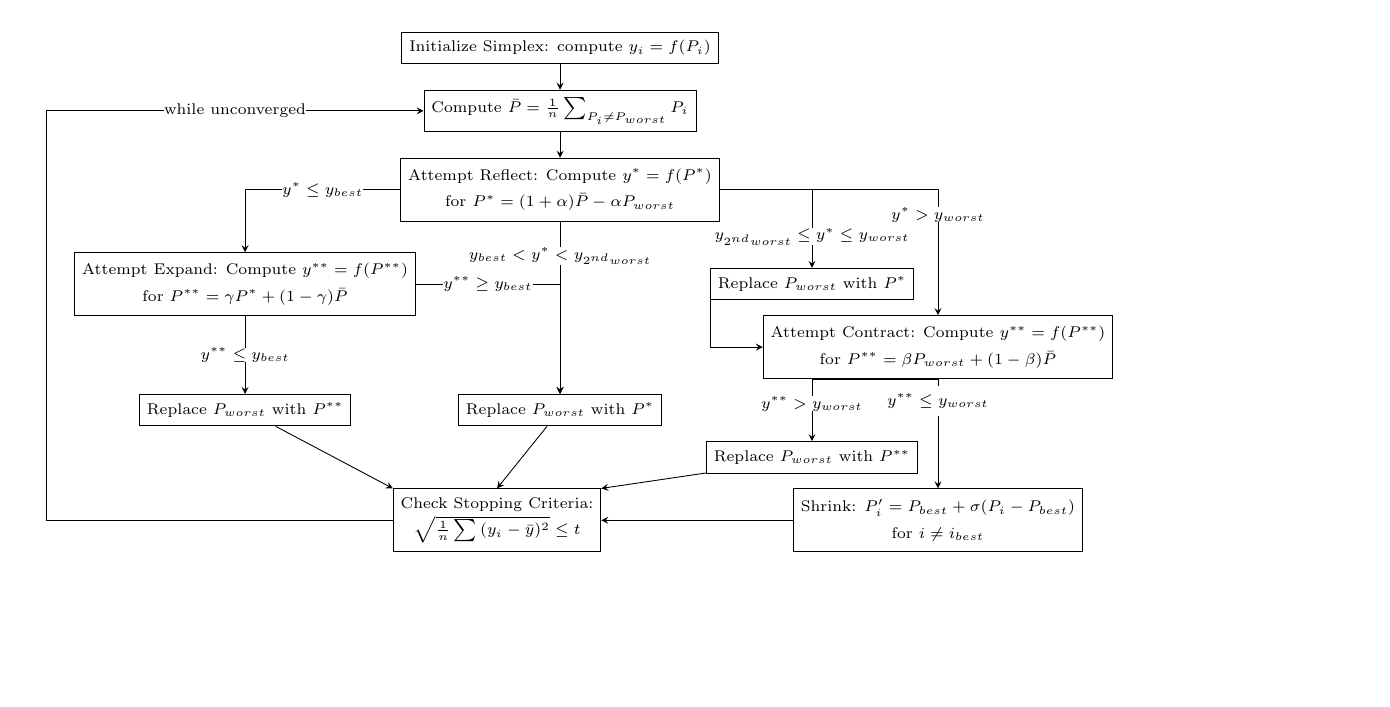
\begin{tikzpicture}
			\scalebox{0.8}{
				\node[draw,minimum height=0.5cm] at (7,0) (init) {\scriptsize Initialize Simplex: compute $y_i=f(P_i)$};
				\node[draw,minimum height=0.5cm] at (7,-1) (pbar) {\scriptsize Compute $\bar{P}=\frac{1}{n}\sum_{P_i\neq P_{worst}}P_i$};
				\node[draw,minimum height=1cm,align=center] at (7,-2.25) (reflect) {\scriptsize Attempt Reflect: Compute $y^*=f(P^*)$ \\ \scriptsize for $P^*=(1+\alpha)\bar{P}-\alpha P_{worst} $};
				\node[draw,minimum height=1cm,align=center] at (2,-3.75) (expand) {\scriptsize Attempt Expand: Compute $y^{**}=f(P^{**})$ \\ \scriptsize for $P^{**}=\gamma P^*+(1-\gamma)\bar{P}$};
				\node[draw,minimum height=.5cm,align=center] at (7,-5.75) (phpstar) {\scriptsize Replace $P_{worst}$ with $P^*$};
				\node[draw,minimum height=.5cm,align=center] at (2,-5.75) (phpstarstar) {\scriptsize Replace $P_{worst}$ with $P^{**}$};
				\node[draw,minimum height=.5cm,align=center] at (11,-3.75) (ystarworst) {\scriptsize  Replace $P_{worst}$ with $P^{*}$};
				\node[draw,minimum height=1cm,align=center] at (13,-4.75) (contract) {\scriptsize Attempt Contract: Compute $y^{**}=f(P^{**})$ \\ \scriptsize for $P^{**}=\beta P_{worst}+(1-\beta)\bar{P}$};
				\node[draw,minimum height=0.5cm,align=center] at (11,-6.5) (phpstarstar2) {\scriptsize Replace $P_{worst}$ with $P^{**}$};
				\node[draw,minimum height=1cm,align=center] at (13,-7.5) (shrink) {\scriptsize Shrink: $P_i'=P_{best}+\sigma(P_i-P_{best})$ \\ \scriptsize for $i\ne i_{best}$};
				\node[draw,minimum height=1cm,align=center] at (6,-7.5) (stop) {\scriptsize Check Stopping Criteria: \\ \scriptsize $ \sqrt{\frac{1}{n}\sum{(y_i-\bar{y})^2}}\le t$};
				
				\draw[-stealth] (init) edge (pbar);
				\draw[-stealth] (pbar) edge (reflect);
				\draw[-stealth] (reflect) -| (expand) node[pos=0.25,fill=white,inner sep=0]{\scriptsize $y^*\leq y_{best}$};
				\draw[-stealth] (expand) -| (phpstar) node[pos=0.25,fill=white,inner sep=0]{\scriptsize $y^{**}\geq y_{best}$};
				\draw[-stealth] (expand.south) -| (phpstarstar.north) node[pos=0.75,fill=white,inner sep=0]{\scriptsize $y^{**}\le y_{best}$};
				\draw[-stealth] (reflect.south) -| (phpstar.north) node[pos=0.6,fill=white,inner sep=0]{\scriptsize $y_{best}<y^*<y_{2^{nd} worst}$};
				\draw[-stealth] (reflect) -| (ystarworst) node[pos=0.8,fill=white,inner sep=0]{\scriptsize $y_{2^{nd} worst} \leq y^* \leq y_{worst}$};
				\draw[-stealth] (reflect) -| (contract) node[pos=0.6,fill=white,inner sep=0]{\scriptsize $y^* > y_{worst}$};
				\draw[-stealth] (ystarworst.west) |- (contract.west);
				\draw[-stealth] (contract.south) -| (phpstarstar2.north) node[pos=0.7,fill=white,inner sep=0]{\scriptsize $y^{**} > y_{worst}$};
				\draw[-stealth] (contract.south) -| (shrink.north) node[pos=0.6,fill=white]{\scriptsize $y^{**} \le y_{worst}$};
				\draw[-stealth] (shrink) edge (stop.east);
				\draw[-stealth] (phpstarstar2) edge (stop.{north east});
				\draw[-stealth] (phpstar) edge (stop.north);
				\draw[-stealth] (phpstarstar) edge (stop.{north west});
				\draw[-stealth]  (stop.west)to++(-5.5,0) |- (pbar.west) node[pos=0.75,fill=white,inner sep=0]{\scriptsize while unconverged};
				
				
			}
			\end{tikzpicture}

	\end{frame}
	
	\begin{frame}
		\frametitle{Motivating Problem: Initialized Simplex}
		\begin{center}
			\begin{tikzpicture} 
				\begin{axis}[extra description/.code={
						\node[anchor=west,align=center] (description1) at (1.1,0.5) 
						{$P_0=\begin{bmatrix} -30 & 30 \end{bmatrix}$ \\ 
							$y_0=f(P_0)=-1.678$ \\ \\
							$P_1=\begin{bmatrix} -20 & 20 \end{bmatrix}$ \\ 
							$y_1=f(P_1)=-6.438$ \\ \\		 				
							$P_2=\begin{bmatrix} -10 & 30 \end{bmatrix}$ \\ 
							$y_2=f(P_2)=-3.718$
						};
					},
					scale=1,
					xmin=-50,xmax=50,
					ymin=-50,ymax=50,
					zmax=0,
					ztick={-10,0},
					xlabel=$x_1$,
					ylabel=$x_2$,
					view={45}{82},]
					\addplot3[surf,domain=-50:50]{-10+.006*(x-1)^2+.009*(y-2)^2+.005*x*y};
					\addplot3[mark=none,thick,black,fill=white,fill opacity=.5] coordinates {(-30,30,-1.678) (-20,20,-6.438) (-10,30,-3.718) (-30,30,-1.678)};
					\addplot3[mark=*,thick,black,text=white,mark options={fill=white, opacity=1, scale=1.5}, nodes near coords, point meta=explicit symbolic,    visualization depends on={value \thisrow{anchor}\as\myanchor},
					every node near coord/.append style={font=\small,anchor=\myanchor}] table [
					row sep=\\,
					meta=label
					]{
						x y z label anchor\\
						-30 30 -1.678 $P_0$ south\\
						-20 20 -6.438 $P_1$ east\\
						-10 30 -3.718 $P_2$ west\\
					};
				\end{axis}
			\end{tikzpicture}
		\end{center}
	\end{frame}

	\begin{frame}
		\frametitle{Motivating Problem: Iteration 1}
		\begin{center}
			\begin{tikzpicture} 
				\begin{axis}[extra description/.code={
						\node[anchor=west,align=center] (description1) at (1.1,0.5) 
						{$P_0=\begin{bmatrix} 0 & 20 \end{bmatrix}$ \\ 
							$y_0=f(P_0)=-7.078$ \\ \\
							$P_1=\begin{bmatrix} -20 & 20 \end{bmatrix}$ \\ 
							$y_1=f(P_1)=-6.438$ \\ \\		 				
							$P_2=\begin{bmatrix} -10 & 30 \end{bmatrix}$ \\ 
							$y_2=f(P_2)=-3.718$
						};
					},
					scale=1,
					xmin=-50,xmax=50,
					ymin=-50,ymax=50,
					zmax=0,
					ztick={-10,0},
					xlabel=$x_1$,
					ylabel=$x_2$,
					view={45}{82},]
					\addplot3[surf,domain=-50:50]{-10+.006*(x-1)^2+.009*(y-2)^2+.005*x*y};
					\addplot3[mark=none,thick,black,fill=white,fill opacity=.5] coordinates {(0,20,-7.078) (-20,20,-6.438) (-10,30,-3.718) (0,20,-7.078)};
					\addplot3[mark=*,thick,black,text=white,mark options={fill=white, opacity=1, scale=1.5}, nodes near coords, point meta=explicit symbolic,    visualization depends on={value \thisrow{anchor}\as\myanchor},
					every node near coord/.append style={font=\small,anchor=\myanchor}] table [
					row sep=\\,
					meta=label
					]{
						x y z label anchor\\
						0 20 -7.078 $P_0$ west\\
						-20 20 -6.438 $P_1$ east\\
						-10 30 -3.718 $P_2$ west\\
					};
				\end{axis}
			\end{tikzpicture}
		\end{center}
	\end{frame}

	\begin{frame}
		\frametitle{Motivating Problem: Iteration 2}
		\begin{center}
			\begin{tikzpicture} 
				\begin{axis}[extra description/.code={
						\node[anchor=west,align=center] (description1) at (1.1,0.5) 
						{$P_0=\begin{bmatrix} 0 & 20 \end{bmatrix}$ \\ 
							$y_0=f(P_0)=-7.078$ \\ \\
							$P_1=\begin{bmatrix} -20 & 20 \end{bmatrix}$ \\ 
							$y_1=f(P_1)=-6.438$ \\ \\		 				
							$P_2=\begin{bmatrix} -10 & 10 \end{bmatrix}$ \\ 
							$y_2=f(P_2)=-9.198$
						};
					},
					scale=1,
					xmin=-50,xmax=50,
					ymin=-50,ymax=50,
					zmax=0,
					ztick={-10,0},
					xlabel=$x_1$,
					ylabel=$x_2$,
					view={45}{82},]
					\addplot3[surf,domain=-50:50]{-10+.006*(x-1)^2+.009*(y-2)^2+.005*x*y};
					\addplot3[mark=none,thick,black,fill=white,fill opacity=.5] coordinates {(0,20,-7.078) (-20,20,-6.438) (-10,10,-9.198) (0,20,-7.078)};
					\addplot3[mark=*,thick,black,text=white,mark options={fill=white, opacity=1, scale=1.5}, nodes near coords, point meta=explicit symbolic,    visualization depends on={value \thisrow{anchor}\as\myanchor},
					every node near coord/.append style={font=\small,anchor=\myanchor}] table [
					row sep=\\,
					meta=label
					]{
						x y z label anchor\\
						0 20 -7.078 $P_0$ west\\
						-20 20 -6.438 $P_1$ east\\
						-10 10 -9.198 $P_2$ east\\
					};
				\end{axis}
			\end{tikzpicture}
		\end{center}
	\end{frame}

	\begin{frame}
		\frametitle{Motivating Problem: Iteration 3}
		\begin{center}
			\begin{tikzpicture} 
				\begin{axis}[extra description/.code={
						\node[anchor=west,align=center] (description1) at (1.1,0.5) 
						{$P_0=\begin{bmatrix} 0 & 20 \end{bmatrix}$ \\ 
							$y_0=f(P_0)=-7.078$ \\ \\
							$P_1=\begin{bmatrix} 10 & 10 \end{bmatrix}$ \\ 
							$y_1=f(P_1)=-8.438$ \\ \\		 				
							$P_2=\begin{bmatrix} -10 & 10 \end{bmatrix}$ \\ 
							$y_2=f(P_2)=-9.198$
						};
					},
					scale=1,
					xmin=-50,xmax=50,
					ymin=-50,ymax=50,
					zmax=0,
					ztick={-10,0},
					xlabel=$x_1$,
					ylabel=$x_2$,
					view={45}{82},]
					\addplot3[surf,domain=-50:50]{-10+.006*(x-1)^2+.009*(y-2)^2+.005*x*y};
					\addplot3[mark=none,thick,black,fill=white,fill opacity=.5] coordinates {(0,20,-7.078) (10,10,-8.438) (-10,10,-9.198) (0,20,-7.078)};
					\addplot3[mark=*,thick,black,text=white,mark options={fill=white, opacity=1, scale=1.5}, nodes near coords, point meta=explicit symbolic,    visualization depends on={value \thisrow{anchor}\as\myanchor},
					every node near coord/.append style={font=\small,anchor=\myanchor}] table [
					row sep=\\,
					meta=label
					]{
						x y z label anchor\\
						0 20 -7.078 $P_0$ west\\
						10 10 -8.438 $P_1$ west\\
						-10 10 -9.198 $P_2$ east\\
					};
				\end{axis}
			\end{tikzpicture}
		\end{center}
	\end{frame}

	\begin{frame}
		\frametitle{Motivating Problem: Iteration 4}
		\begin{center}
			\begin{tikzpicture} 
				\begin{axis}[extra description/.code={
						\node[anchor=west,align=center] (description1) at (1.1,0.5) 
						{$P_0=\begin{bmatrix} 0 & 0 \end{bmatrix}$ \\ 
							$y_0=f(P_0)=-9.958$ \\ \\
							$P_1=\begin{bmatrix} 10 & 10 \end{bmatrix}$ \\ 
							$y_1=f(P_1)=-8.438$ \\ \\		 				
							$P_2=\begin{bmatrix} -10 & 10 \end{bmatrix}$ \\ 
							$y_2=f(P_2)=-9.198$
						};
					},
					scale=1,
					xmin=-50,xmax=50,
					ymin=-50,ymax=50,
					zmax=0,
					ztick={-10,0},
					xlabel=$x_1$,
					ylabel=$x_2$,
					view={45}{82},]
					\addplot3[surf,domain=-50:50]{-10+.006*(x-1)^2+.009*(y-2)^2+.005*x*y};
					\addplot3[mark=none,thick,black,fill=white,fill opacity=.5] coordinates {(0,0,-9.958) (10,10,-8.438) (-10,10,-9.198) (0,0,-9.958)};
					\addplot3[mark=*,thick,black,text=white,mark options={fill=white, opacity=1, scale=1.5}, nodes near coords, point meta=explicit symbolic,    visualization depends on={value \thisrow{anchor}\as\myanchor},
					every node near coord/.append style={font=\small,anchor=\myanchor}] table [
					row sep=\\,
					meta=label
					]{
						x y z label anchor\\
						0 0 -9.958 $P_0$ west\\
						10 10 -8.438 $P_1$ west\\
						-10 10 -9.198 $P_2$ east\\
					};
				\end{axis}
			\end{tikzpicture}
		\end{center}
	\end{frame}
	
	\begin{frame}
		\frametitle{Motivating Problem: Iteration 5}
		\begin{center}
			\begin{tikzpicture} 
				\begin{axis}[extra description/.code={
						\node[anchor=west,align=center] (description1) at (1.1,0.5) 
						{$P_0=\begin{bmatrix} 0 & 0 \end{bmatrix}$ \\ 
							$y_0=f(P_0)=-9.958$ \\ \\
							$P_1=\begin{bmatrix} -7.5 & -2.5 \end{bmatrix}$ \\ 
							$y_1=f(P_1)=-9.291$ \\ \\		 				
							$P_2=\begin{bmatrix} -10 & 10 \end{bmatrix}$ \\ 
							$y_2=f(P_2)=-9.198$
						};
					},
					scale=1,
					xmin=-50,xmax=50,
					ymin=-50,ymax=50,
					zmax=0,
					ztick={-10,0},
					xlabel=$x_1$,
					ylabel=$x_2$,
					view={45}{82},]
					\addplot3[surf,domain=-50:50]{-10+.006*(x-1)^2+.009*(y-2)^2+.005*x*y};
					\addplot3[mark=none,thick,black,fill=white,fill opacity=.5] coordinates {(0,0,-9.958) (-7.5,-2.5,-9.2905) (-10,10,-9.198) (0,0,-9.958)};
					\addplot3[mark=*,thick,black,text=white,mark options={fill=white, opacity=1, scale=1.5}, nodes near coords, point meta=explicit symbolic,    visualization depends on={value \thisrow{anchor}\as\myanchor},
					every node near coord/.append style={font=\small,anchor=\myanchor}] table [
					row sep=\\,
					meta=label
					]{
						x y z label anchor\\
						0 0 -9.958 $P_0$ west\\
						-7.5 -2.5 -9.2905 $P_1$ east\\
						-10 10 -9.198 $P_2$ east\\
					};
				\end{axis}
			\end{tikzpicture}
		\end{center}
	\end{frame}

	\begin{frame}
		\frametitle{Motivating Problem: Iteration 6}
		\begin{center}
			\begin{tikzpicture} 
				\begin{axis}[extra description/.code={
						\node[anchor=west,align=center] (description1) at (1.1,0.5) 
						{$P_0=\begin{bmatrix} 0 & 0 \end{bmatrix}$ \\ 
							$y_0=f(P_0)=-9.958$ \\ \\
							$P_1=\begin{bmatrix} -7.5 & -2.5 \end{bmatrix}$ \\ 
							$y_1=f(P_1)=-9.291$ \\ \\		 				
							$P_2=\begin{bmatrix} 3.13 & -5.63 \end{bmatrix}$ \\ 
							$y_2=f(P_2)=-9.538$
						};
					},
					scale=1,
					xmin=-50,xmax=50,
					ymin=-50,ymax=50,
					zmax=0,
					ztick={-10,0},
					xlabel=$x_1$,
					ylabel=$x_2$,
					view={45}{82},]
					\addplot3[surf,domain=-50:50]{-10+.006*(x-1)^2+.009*(y-2)^2+.005*x*y};
					\addplot3[mark=none,thick,black,fill=white,fill opacity=.5] coordinates {(0,0,-9.958) (-7.5,-2.5,-9.2905) (3.125,-5.625,-9.537531) (0,0,-9.958)};
					\addplot3[mark=*,thick,black,text=white,mark options={fill=white, opacity=1, scale=1.5}, nodes near coords, point meta=explicit symbolic,    visualization depends on={value \thisrow{anchor}\as\myanchor},
					every node near coord/.append style={font=\small,anchor=\myanchor}] table [
					row sep=\\,
					meta=label
					]{
						x y z label anchor\\
						0 0 -9.958 $P_0$ west\\
						-7.5 -2.5 -9.2905 $P_1$ east\\
						3.125 -5.625 -9.537531 $P_2$ east\\
					};
				\end{axis}
			\end{tikzpicture}
		\end{center}
	\end{frame}

	\begin{frame}
		\frametitle{Motivating Problem: Iteration 7}
		\begin{center}
			\begin{tikzpicture} 
				\begin{axis}[extra description/.code={
						\node[anchor=west,align=center] (description1) at (1.1,0.5) 
						{$P_0=\begin{bmatrix} 0 & 0 \end{bmatrix}$ \\ 
							$y_0=f(P_0)=-9.958$ \\ \\
							$P_1=\begin{bmatrix} -4.53 & .156 \end{bmatrix}$ \\ 
							$y_1=f(P_1)=-9.789$ \\ \\		 				
							$P_2=\begin{bmatrix} 3.13 & -5.63 \end{bmatrix}$ \\ 
							$y_2=f(P_2)=-9.538$
						};
					},
					scale=1,
					xmin=-50,xmax=50,
					ymin=-50,ymax=50,
					zmax=0,
					ztick={-10,0},
					xlabel=$x_1$,
					ylabel=$x_2$,
					view={45}{82},]
					\addplot3[surf,domain=-50:50]{-10+.006*(x-1)^2+.009*(y-2)^2+.005*x*y};
					\addplot3[mark=none,thick,black,fill=white,fill opacity=.5] coordinates {(0,0,-9.958) (-4.53125,.156250,-9.789377) (3.125,-5.625,-9.537531) (0,0,-9.958)};
					\addplot3[mark=*,thick,black,text=white,mark options={fill=white, opacity=1, scale=1.5}, nodes near coords, point meta=explicit symbolic,    visualization depends on={value \thisrow{anchor}\as\myanchor},
					every node near coord/.append style={font=\small,anchor=\myanchor}] table [
					row sep=\\,
					meta=label
					]{
						x y z label anchor\\
						0 0 -9.958 $P_0$ west\\
						-4.53125 .156250 -9.789377 $P_1$ east\\
						3.125 -5.625 -9.537531 $P_2$ east\\
					};
				\end{axis}
			\end{tikzpicture}
		\end{center}
	\end{frame}

	\begin{frame}
		\frametitle{Motivating Problem: Convergence History}
		\begin{center}
		\begin{tabular}{||c c c c||c c||} 
			\hline
			Iter. & Func Evals & $y_{best}$ & $P_{best}$ & $Error(y_{best})$ & $Error(P_{best})$ \\ [0.5ex] 
			\hline\hline
			1 & 5 & -7.078000 & $\begin{bmatrix} 0 & 20 \end{bmatrix}$ & 2.916188 & $\begin{bmatrix} -0.188 & 18.052 \end{bmatrix}$ \\ 
			\hline
			2 & 7 & -9.198000 & $\begin{bmatrix} -10 & 10 \end{bmatrix}$ & 0.796188 & $\begin{bmatrix} -10.188 & 8.052 \end{bmatrix}$  \\
			\hline
			3 & 8 & -9.198000 & $\begin{bmatrix} -10 & 10 \end{bmatrix}$ & 0.796188 & $\begin{bmatrix} -10.188 & 8.052 \end{bmatrix}$\\
			\hline
			4 & 10 & -9.958000 & $\begin{bmatrix} 0 & 0 \end{bmatrix}$ & 0.036188 & $\begin{bmatrix} -0.188 & -1.948 \end{bmatrix}$\\
			\hline
			5 & 12 & -9.958000 & $\begin{bmatrix} 0 & 0 \end{bmatrix}$ & 0.036188 & $\begin{bmatrix} -0.188 & -1.948 \end{bmatrix}$\\ 
			\hline
			... & ... & ... & ... & ... & ... \\ 
			\hline
			10 & 22 & -9.994024 & $\begin{bmatrix} 0.2441 & 2.0605 \end{bmatrix}$ & 0.000164 & $\begin{bmatrix} 0.056 & 0.113 \end{bmatrix}$ \\ 			
			\hline
			... & ... & ... & ... & ... & ... \\ 
			\hline
			15 & 42 & -9.994180 & $\begin{bmatrix} 0.2288 & 1.9317 \end{bmatrix}$ & 0.000008 & $\begin{bmatrix} 0.040 & -0.016 \end{bmatrix}$ \\ 
			\hline
			... & ... & ... & ... & ... & ... \\ 
			\hline
			20 & 59 & -9.994188 & $\begin{bmatrix} 0.1891 & 1.9466 \end{bmatrix}$ & 0.0000005 & $\begin{bmatrix} 0.001 & -0.001 \end{bmatrix}$ \\ 			
			\hline
			... & ... & ... & ... & ... & ... \\ 
			\hline
			25 & 76 & -9.994188 & $\begin{bmatrix} 0.1885 & 1.9475 \end{bmatrix}$ & 0.0000005 & $\begin{bmatrix} 0.0001 & -0.0001 \end{bmatrix}$ \\ 
			\hline
		\end{tabular}
		
		\end{center}
	\end{frame}

	\begin{frame}
		\frametitle{Concluding Remarks}
		Pros of Nelder-Mead:
		\begin{itemize}
			\item easy to understand and implement programmatically
			\item no need to compute derivatives (non differentiable functions)
			\item only need to track $n+1$ data points
			\item low amount of function evaluations per iteration (not counting \textbf{SHRINK} step)
		\end{itemize}
		\vspace{1cm}
		Cons of Nelder-Mead:
		\begin{itemize}
			\item may sometimes be slow to converge or may fail entirely
			\item no way to ensure global optimum (not unique to NM)
		\end{itemize}
	\end{frame}

	\begin{frame}
		\frametitle{Concluding Remarks (cont)}
			This implementation was ``unconstrained optimization" without constraints on the design variables or boundaries on the design space. Constraints can be imposed within the objective function with relative ease (see ``Penalty Methods", etc.). That is out of the scope of this document.
			\\[\baselineskip] 
			It is also possible to impose simple boundary constraints on the design variables within the algorithm itself. Can you think of an easy way to do this?
	\end{frame}
\end{document}
